% Instructions to change to html version:
% Comment out:
%  minipage, multicols,columnbreak, mathbf, hrule
% Replace all: \begin{minipage}% %%\end{minipage} %%%%\begin{mulicols}  %%%%\end{mulicols}  %%%\columnbreak % %%%\begin{framed} %%%%\end{framed} %%%%\hrule
% Search for \mathbf
% Replace \\] with \[ and \) with \(
% Enclose graphics in figure environments and add captions
% Re-tag \df environments as sections, subsections, etc.
% Command Line Code to Create html version:
%First: pdflatex -shell-escape filename.tex                                   
%Second, for each figure: inkscape "filename-figure1.pdf" -o "filename-figure1.png"
% Third: htlatex filename.tex "ht5mjlatex.cfg, charset=utf-8" " -cunihtf -utf8"


\documentclass[10pt]{article}

%\usepackage{tikz, pgf,pgfplots,wasysym,array}
%\usepackage{wasysym,array}

\usepackage{amsmath,amssymb}

\ifdefined\HCode
  \def\pgfsysdriver{pgfsys-tex4ht-updated.def}
\fi 
%\ifdefined\HCode
%  \def\pgfsysdriver{pgfsys-dvisvgm4ht.def}
%\fi 
\usepackage{tikz}
\usetikzlibrary{calc,decorations.markings,arrows}
\usepackage{pgfplots}

\pgfplotsset{compat=1.12}
\usepackage{myexternalize}
\usetikzlibrary{calc,decorations.markings,arrows}
\usepackage{framed}
\usepackage[none]{hyphenat}

\input{../../../common/1336_header_test.tex}

\begin{document}


\renewcommand{\myTitle}{MATH 2330: Multivariable Calculus}

\renewcommand{\mySubTitle}{4.3: Partial Derivatives}
%~\hfill Name: \underline{~~~~~~~~~~~~~~~~~~~~~~~~~~~~~~~~~~~~~~~~~~~~~~~}

\lectTitle{\vspace*{-.5in}\myTitle}{\vspace*{.1in}\mySubTitle \vspace*{-.25in}}

\rfoot{{\texttt{Page \thepage~of 2}}}

\section*{Section 4.3 -  Partial Derivatives:}

\hspace*{-.8in}%\begin{minipage}{1.25\textwidth}
%\begin{framed}

\subsection*{Definitions \& Terminology:}
%\begin{multicols}{2}
\begin{figure}[!h]
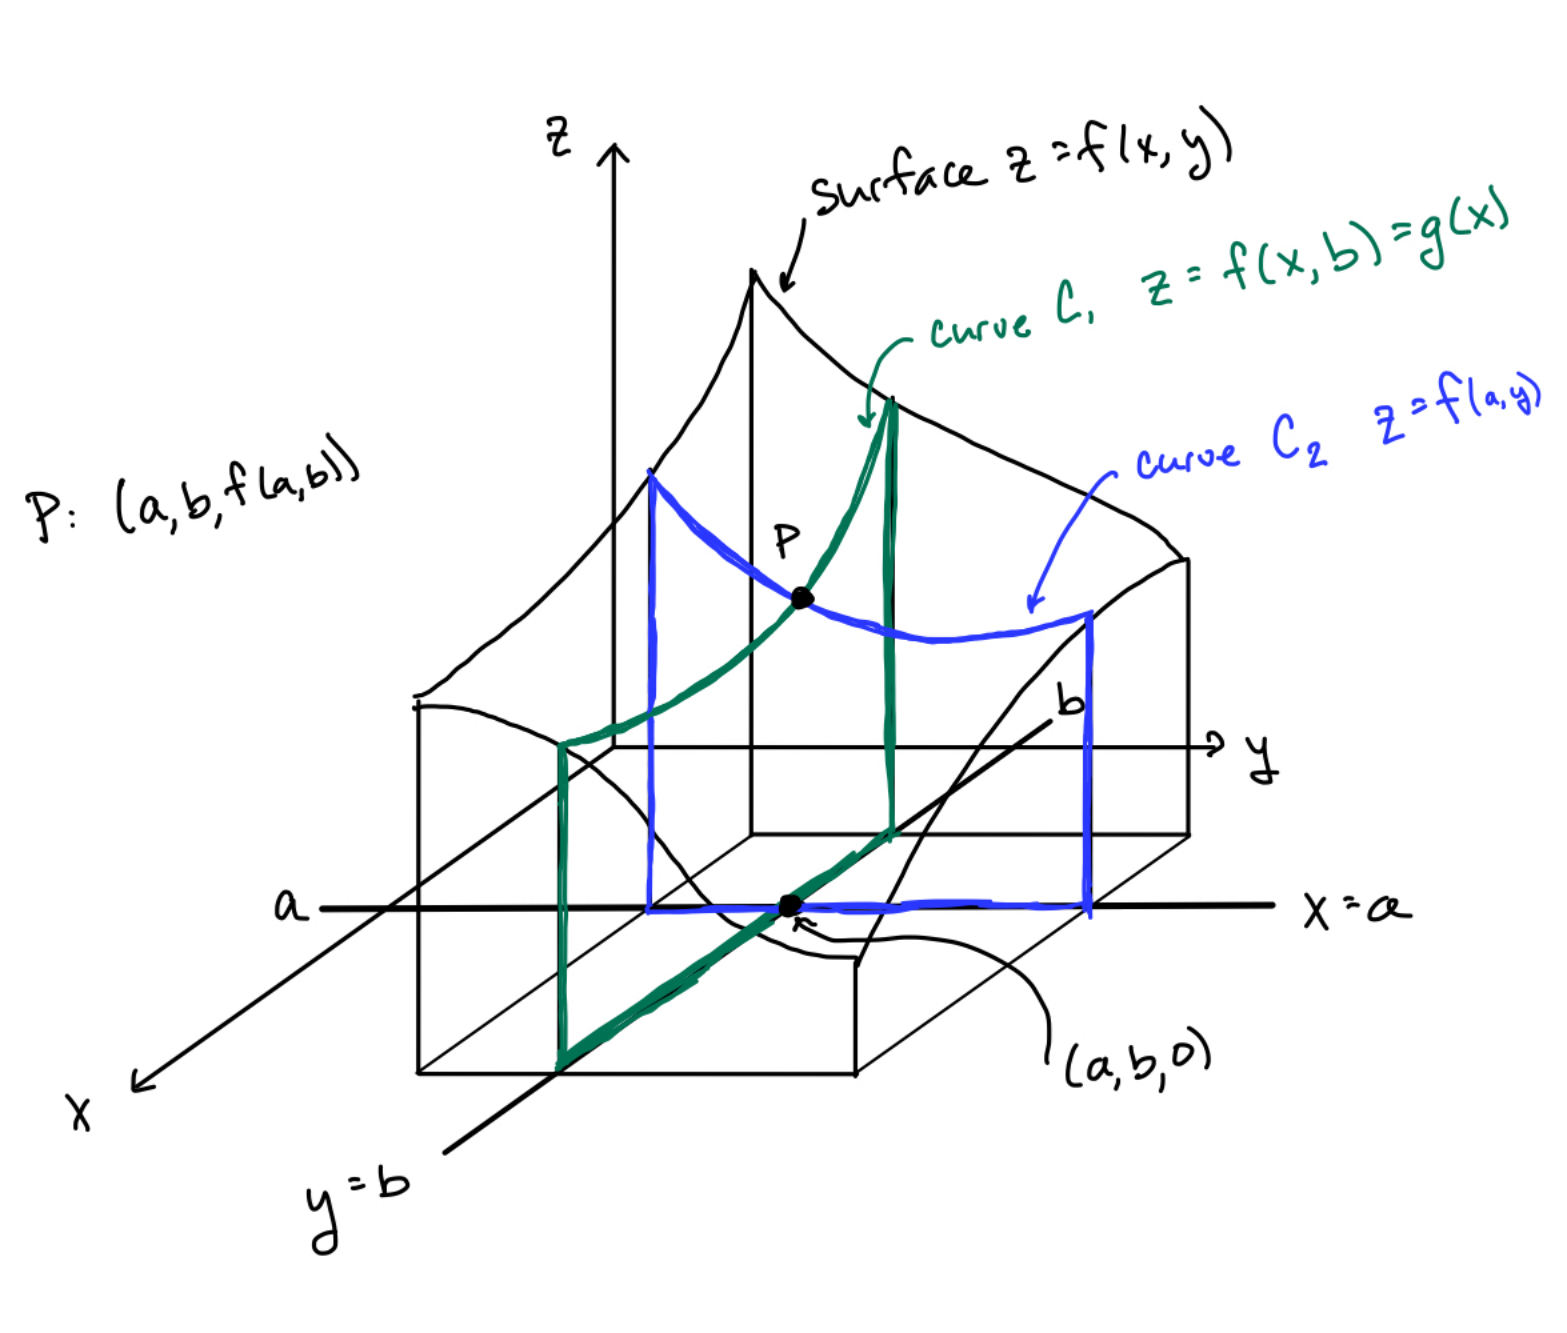
\includegraphics[width=.5\textwidth]{Partial-Derivatives-Geometry.png}
\caption{Partial Derivatives Geometry Diagram}
\end{figure}

%\begin{itemize}
%\item 
The \textbf{partial derivative of \(f\) with respect to \(x\) at the point \((a,b)\)}, \(f_x (a,b)\), is the slope of the line tangent to the curve \(z=f(x,b)\) at the point \((a,b)\).
\begin{itemize}
\item \underline{To compute \(f_x\):}\\ treat \(y\) as a constant, and take the derivative w.r.t. \(x\).
\end{itemize}
%\item 
The \textbf{partial derivative of \(f\) with respect to \(y\) at the point \((a,b)\)}, \(f_y (a,b)\), is the slope of the line tangent to the curve \(z=f(a,y)\) at the point \((a,b)\).
\begin{itemize}
\item \underline{To compute \(f_y\):}\\ treat \(x\) as a constant, and take the derivative w.r.t. \(y\).
\end{itemize}
%\item 
Common types of partial derivative notation:
\[ f_x (x,y) = f_x = \frac{\partial f}{\partial x} = \frac{\partial}{\partial x} f(x,y) = \frac{\partial z}{\partial x}\]
%\end{itemize}
%\end{multicols}

%\hrule
\vspace*{.2in}

\df{\textcolor{sblack}{Clairaut's Theorem:}}

Suppose  \(f\) is defined on a disk \(D\) that contains the point \( (a,b) \).
If the functions \(f_{xy}\) and \(f_{yx}\) are both \textit{continuous} on \(D\), then

\[f_{xy}(a,b) = f_{yx}(a,b)\]

\textbf{Punchline:} If the mixed partial derivatives are continuous, order doesn't matter!

%\end{framed}

%\end{minipage}



\begin{enumerate}[{Example} 1: ]
\item Consider \(f(x,y)=5x^2-2xy+3y^3\). Find \(f_{xy}\) and \(f_{yx}\) and verify that the conclusion of Clairaut's Theorem holds.
\vspace*{.5in}

\item Use implicit differentiation to find \(\dfrac{\partial z}{\partial x}\):

\[x^2-y^2+z^2-2z = 4\]

%\vspace*{.25in}

\end{enumerate}

%\pagebreak


\section*{Section 4.3 Group Work:}

\begin{figure}[!h]

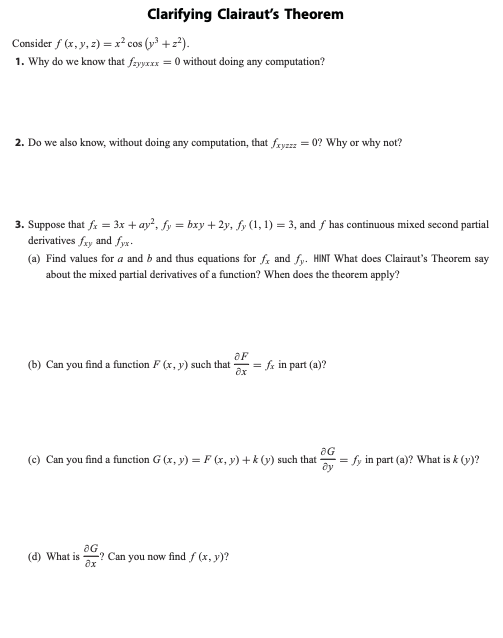
\includegraphics[]{Clarifying-Clairaut.png}
\caption{Clarifying Clairaut Group Work Activity}
\end{figure}

%\pagebreak
%\(~\)
%\vspace*{-.5in}

%
%%\vspace*{-.5in}
%\section*{Section 11.4 - Tangent Planes \& Linear Approximation, Part 1:}
%
%\hspace*{-.8in}%\begin{minipage}{1.25\textwidth}
%%\begin{framed}
%
%\df{\textcolor{sblack}{Definitions \& Terminology:}}
%\begin{multicols}{2}
%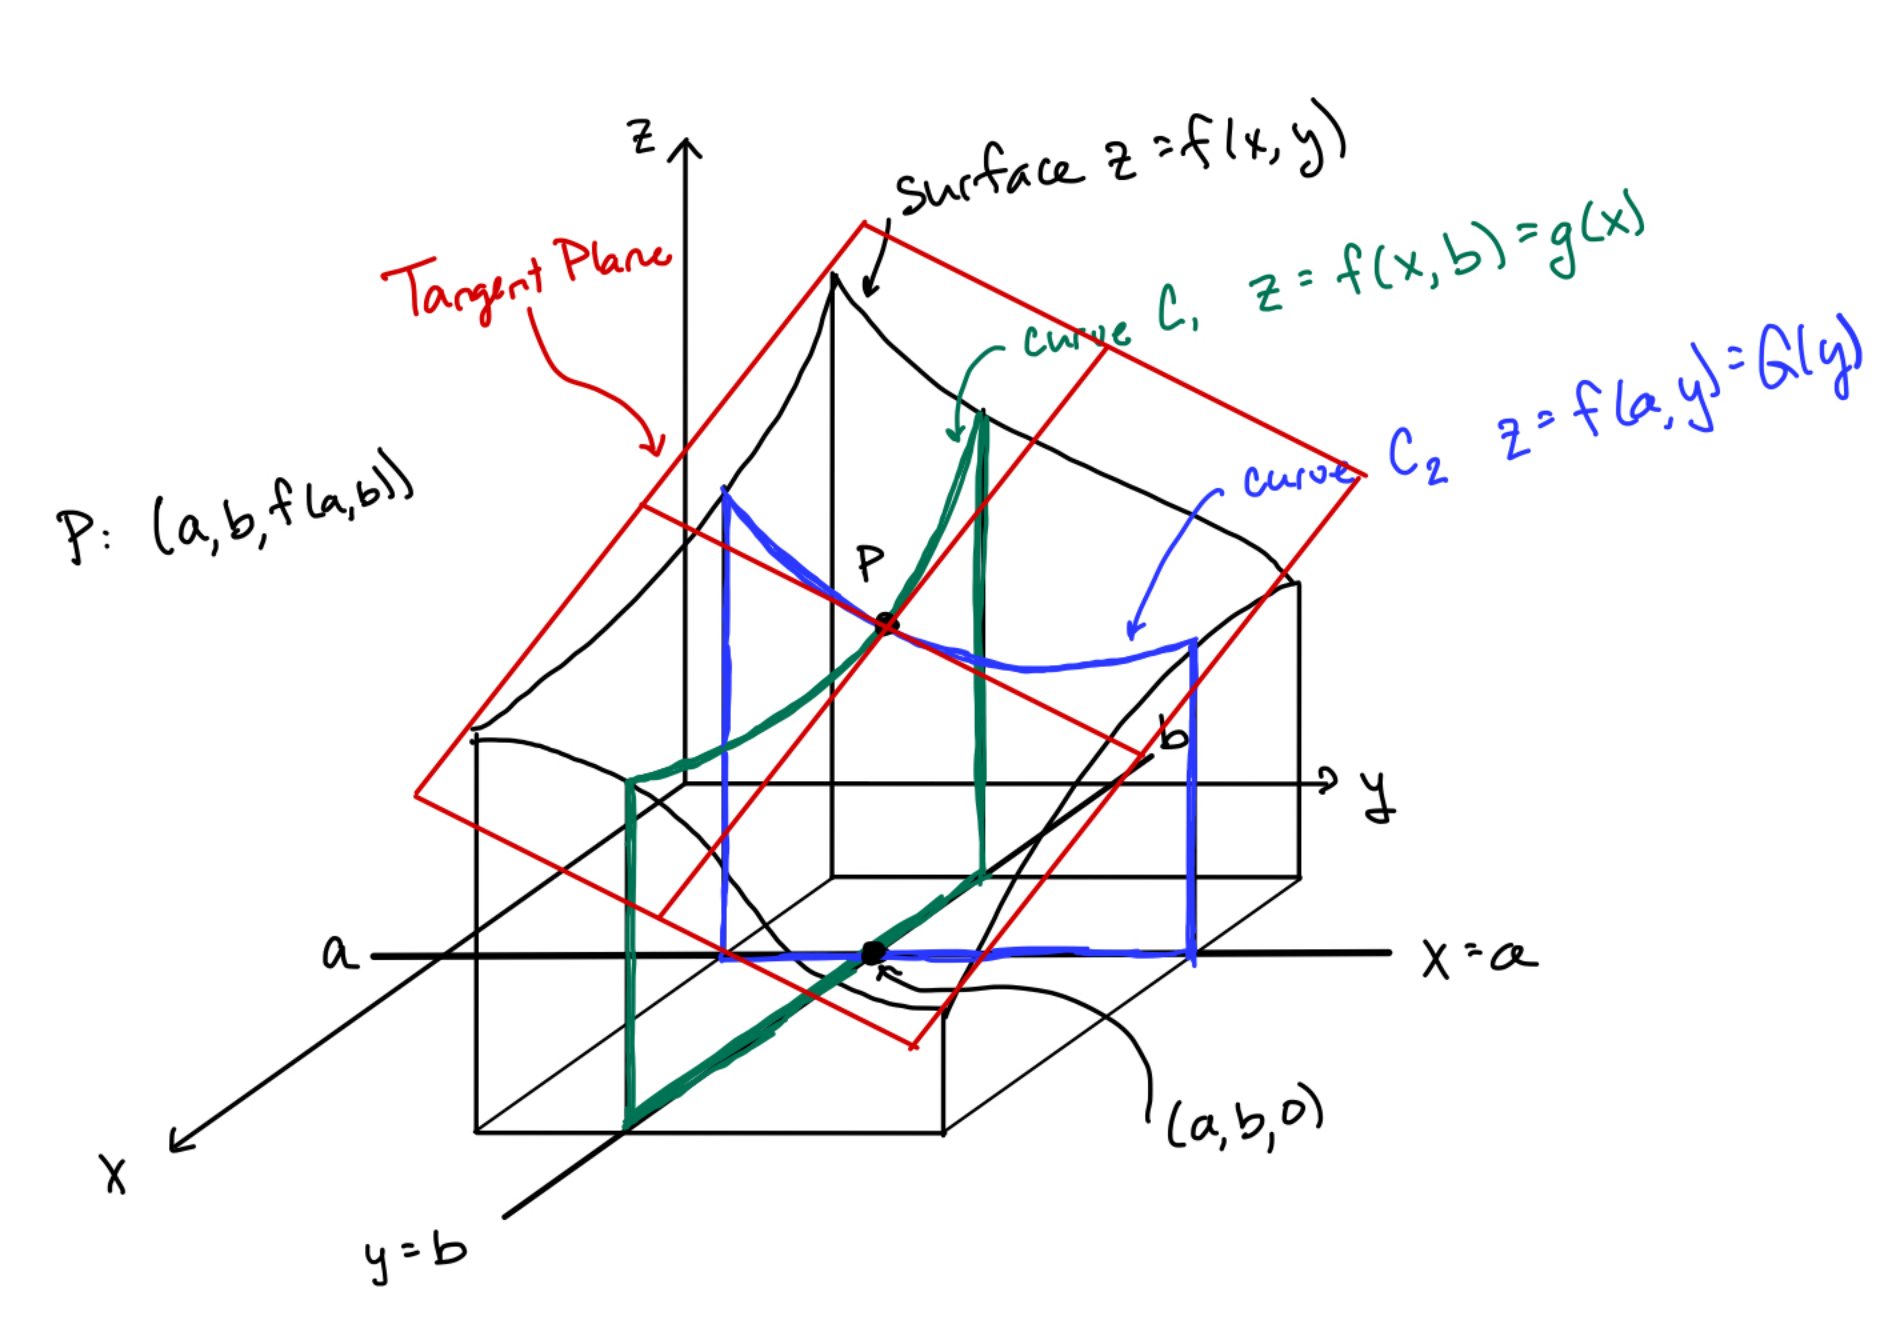
\includegraphics[width=\columnwidth]{Tangent-Plane.jpeg}
%
%The \textbf{tangent plane} to the surface \(z=f(x,y)\) at the point \((a,b)\) is the plane defined by the tangent lines in the \(x-\) and \(y-\) directions at the point \((a,b)\).\\
%
%The tangent plane gives the most accurate planar approximation to the surface at the point \((a,b)\).\\
%
%\textbf{Tangent Plane Equation:}
%\[z = f(a,b) + f_x(a,b)(x-a) + f_y(a,b)(y-b)\]
%
%\textbf{Linearization of \(f\) at \((a,b)\):}
%\[L(x,y) = f(a,b) + f_x(a,b)(x-a) + f_y(a,b)(y-b)\]
%
%\textbf{Linear Approximation or Tangent Plane Approximation:}
%\[f(x,y) \approx L(x,y) \]
%
%\end{multicols}
%
%
%%\end{framed}
%
%%\end{minipage}

%
%
%
%\begin{enumerate}[{Example} 1: ]
%\item Consider the function \(f(x,y) = x^2y^3\).
%\begin{enumerate}[(a)]
%\item Find the equation of the tangent plane to \(z=f(x,y)\) at the point \((3,1,9)\).
%\item Use Linear Approximation to estimate the value of \(f(x,y)\) at the point \((2.5,1.5)\).
%\end{enumerate}
%
%\end{enumerate}

\end{document}

